\section{lib/views/qrotorview.cc \-File \-Reference}
\label{qrotorview_8cc}\index{lib/views/qrotorview.\-cc@{lib/views/qrotorview.\-cc}}
{\ttfamily \#include \char`\"{}\-G\-L/glut.\-h\char`\"{}}\*
{\ttfamily \#include $<$assert.\-h$>$}\*
{\ttfamily \#include $<$stdlib.\-h$>$}\*
{\ttfamily \#include $<$string.\-h$>$}\*
{\ttfamily \#include $<$iostream$>$}\*
{\ttfamily \#include \char`\"{}qrotorview.\-h\char`\"{}}\*
{\ttfamily \#include \char`\"{}viewer.\-h\char`\"{}}\*
{\ttfamily \#include \char`\"{}so3.\-h\char`\"{}}\*
{\ttfamily \#include \char`\"{}utils.\-h\char`\"{}}\*
\-Include dependency graph for qrotorview.\-cc\-:\nopagebreak
\begin{figure}[H]
\begin{center}
\leavevmode
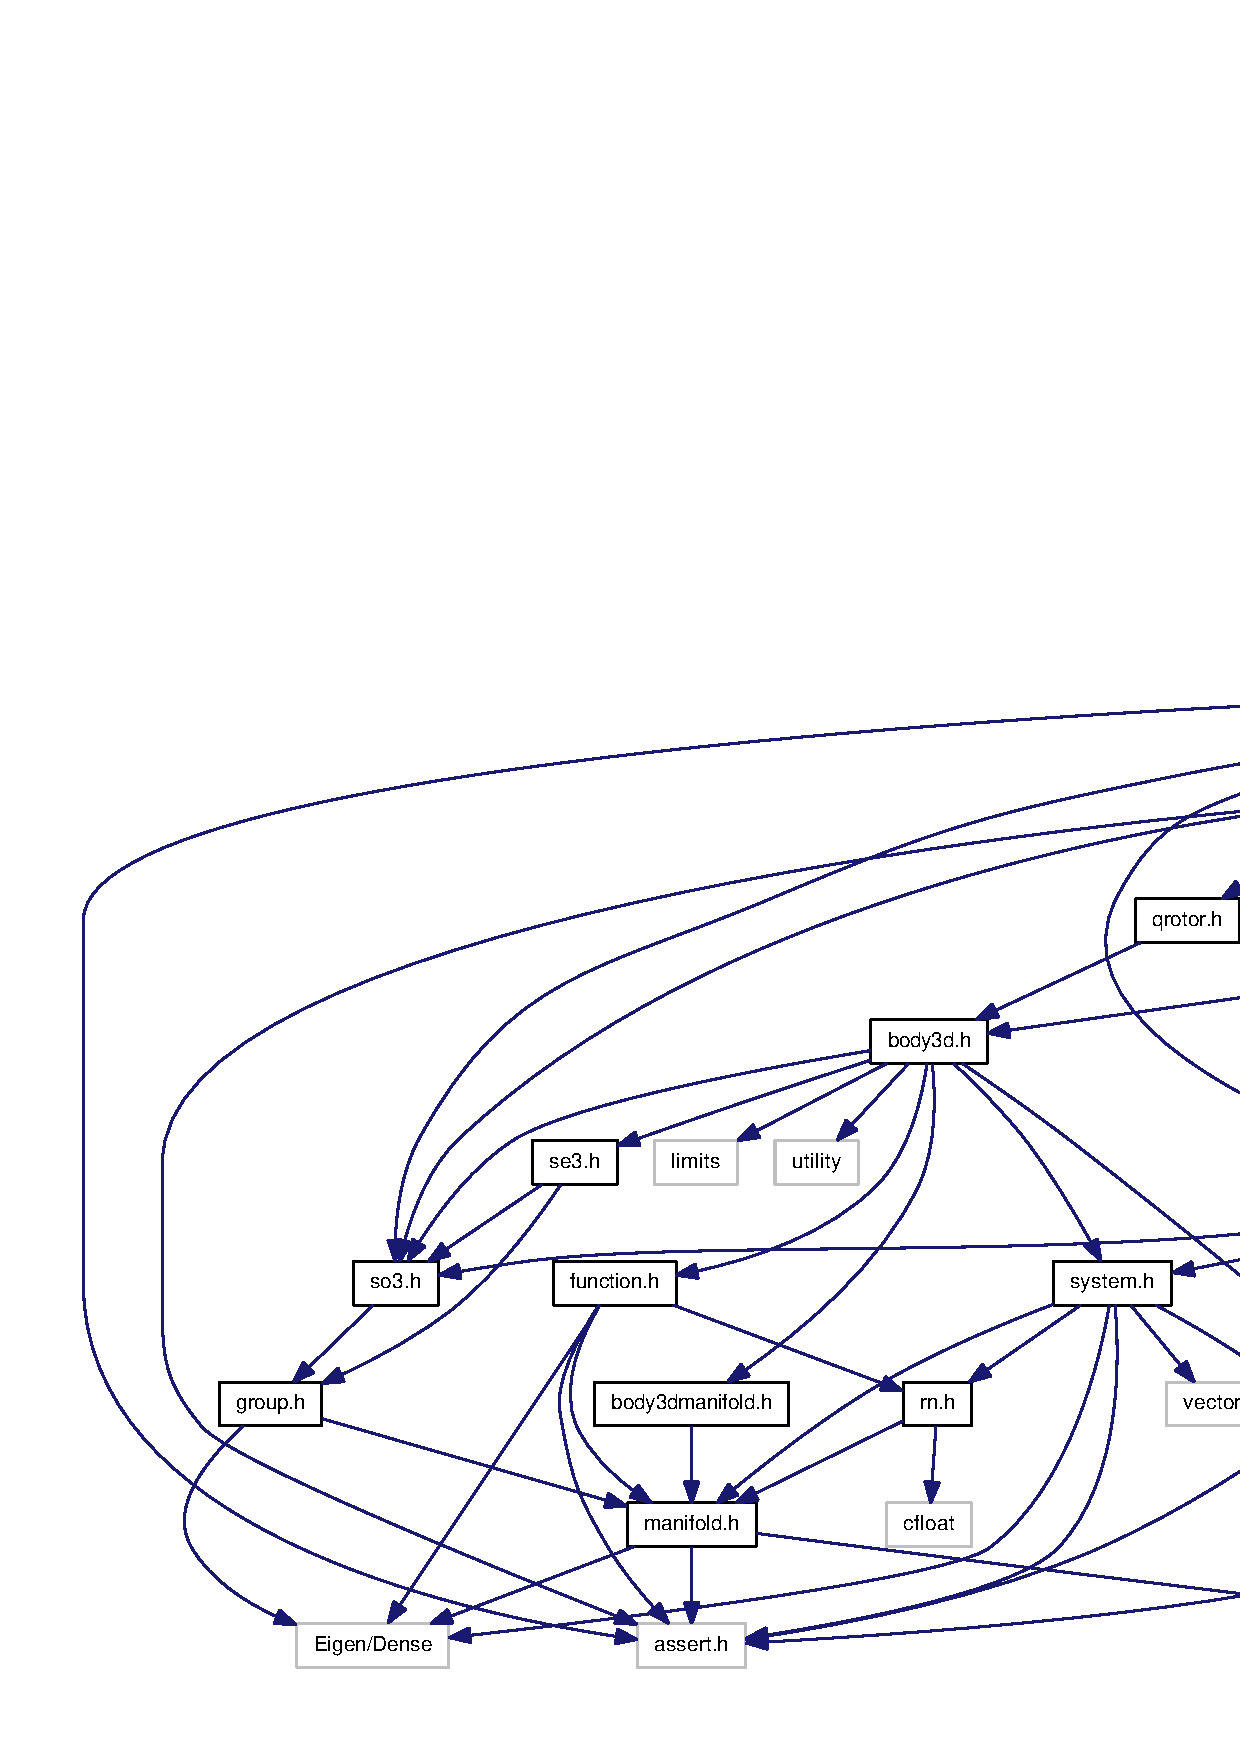
\includegraphics[width=350pt]{qrotorview_8cc__incl}
\end{center}
\end{figure}
